\documentclass[11pt,a4paper]{article}
\usepackage[utf8]{inputenc}
\usepackage[dutch]{babel}
\usepackage{pgfplots}
\usepgfplotslibrary{units}
\usepackage{float}
\usepackage{amsmath,amsthm}
\usepackage{amsfonts}
\usepackage{amssymb}
\usepackage[left=2cm,right=2cm,top=2.5cm,bottom=2cm]{geometry}
\usepackage{graphicx}
\usepackage{multicol}
\usepackage{enumerate}
\usepackage{fancyhdr}
\pagestyle{fancy}
\usepackage{algorithm}
\usepackage{algpseudocode}
\usepackage{pgfplots}
\usepackage{multirow}
\usepackage{tikz}
\usetikzlibrary{calc}

\floatname{algorithm}{Algoritme}


\usepackage[font=small,labelfont=bf]{caption}
\captionsetup[table]{aboveskip=-0.8em}
\captionsetup[table]{belowskip=-0.7pt}


\lhead {DAIII Project: punten plaatsen} 
\chead{BAZ(~ \thepage ~ )NGA} 
\rhead{Robbert Gurdeep Singh}


\cfoot{} % get rid of the page number 

\usepackage{hyperref}
\usepackage{chngcntr}
\counterwithin*{section}{part}
\counterwithin{algorithm}{section}
\counterwithin{table}{section}
\counterwithin{figure}{section}

\hypersetup{
    colorlinks=false,
    pdfborder={0 0 0},
}

\author{Robbert Gurdeep Singh}
\title{{Project Algoritmen en datastructuren III}\\ \Huge Genetische algoritmen}
%\date{}



\pgfplotsset{compat=1.8}


\newcommand{\drawGraph}[4]{
\begin{tikzpicture}
\begin{axis}[scale only axis, 
	%x-as	
    xmin=0,
	xlabel=#1,	
	%y-as
	ylabel=#2,
	ymin=0,
	%Style
	height=5em,width=.37\textwidth,
	enlargelimits=0.05,
	grid=major,	legend pos=south east
]
#3
\end{axis}
\end{tikzpicture}
}


\newcommand{\lxaxis}[3]{\begin{tikzpicture}
\begin{axis}[scale only axis, 
cycle list name=exotic,
    xmode=log,
    log ticks with fixed point,
	%x-as	
	xlabel=#2,	
	%y-as
	ylabel=#1,
	ymin=0,
	%Style
	height=5em,width=.37\textwidth,
	enlargelimits=0.05,
	grid=major,	legend pos=south east
]
#3

\end{axis}
\end{tikzpicture}}

\newcommand{\rlxaxis}[3]{\begin{tikzpicture}
\begin{axis}[scale only axis, 
cycle list name=exotic,
    xmode=log,
    log ticks with fixed point,
	%x-as	
	xlabel=#2,	
	%y-as
	ylabel=#1,
	%Style
	height=5em,width=.37\textwidth,
	enlargelimits=0.05,
	grid=major,	legend pos=south east
]
#3

\end{axis}
\end{tikzpicture}}

\newcommand{\nxaxis}[3]{\begin{tikzpicture}
\begin{axis}[scale only axis,
cycle list name=exotic, 
	%x-as	
    xmin=0,
	xlabel=#2,	
	%y-as
	ylabel=#1,
	ymin=0,
	%Style
	height=5em,width=.37\textwidth,
	enlargelimits=0.05,
	grid=major,	legend pos=south east
]
#3

\end{axis}
\end{tikzpicture}}


\newcommand{\rnxaxis}[3]{\begin{tikzpicture}
\begin{axis}[scale only axis, 
cycle list name=exotic,
	%x-as	
    xmin=0,
	xlabel=#2,	
	%y-as
	ylabel=#1,
	%Style
	height=5em,width=.37\textwidth,
	enlargelimits=0.05,
	grid=major,	legend pos=south east
]
#3

\end{axis}
\end{tikzpicture}}

\newcommand{\itemMB}[1]{
	\item[$\boldsymbol{#1}$:]
}




\newcommand{\abs}[1]{
	\lvert #1 \rvert
}

\newcommand{\addploti}[1]{\addplot table [y=i, x=testValue, col sep=comma] {../../tests/param_results/#1.log};}
\newcommand{\addplotf}[1]{\addplot table [y=f, x=testValue, col sep=comma] {../../tests/param_results/#1.log};}
\newcommand{\addplott}[1]{\addplot table [y=t, x=testValue, col sep=comma] {../../tests/param_results/#1.log};}

\definecolor{mymark}{HTML}{EBB8B8}

\begin{document}

\twocolumn[\begin{@twocolumnfalse}
    \maketitle
\end{@twocolumnfalse}]
\section{Algoritmen}
\label{sec:algoritmen}

\subsection{Punt in veelhoek}
\label{sub:algo-pt-in-poly}
Eén van de voorwaarden waaraan een oplossing moet voldoen is dat alle punten \textbf{in} de veelhoek liggen.Het is dus noodzakelijk om een algoritme te hebben dat bepaalt of een punt zich al dan niet in de convexe veelhoek bevind.
\subsubsection{Idee}
Trekken we een lijn vanuit het punt ``naar boven'', dan kunnen we 3 gevallen onderscheiden:
\begin{itemize}
\item We snijden de veelhoek niet ($P_{1}$): \\
		We weten dat we ons niet binnen de veelhoek bevonden.
\item We snijden de veelhoek juist 1 keer ($P_{2}$):\\
		Nu zijn we zeker in de veelhoek. 
\item We snijden de veelhoek juist\footnote{Merk op dat indien we de veelhoek meer dan 2 keer snijden, we kunnen aantonen dat de veelhoek niet convex is.} 2 keer ($P_{3}$):\\
		We liggen onder en dus ook buiten de veelhoek.
\end{itemize}

\begin{center}
\begin{figure}[H]
\centering
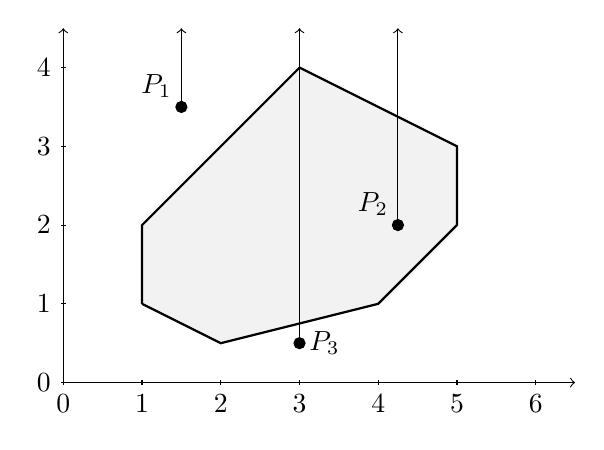
\begin{tikzpicture}
\draw[->] (0,0) -- (6.5,0);
\draw[->] (0,0) -- (0,4.5);

\foreach \x in {0,1,2,3,4,5,6}
    \draw (\x cm,1pt) -- (\x cm,-1pt) node[anchor=north] {\x};
\foreach \y in {0,1,2,3,4}
    \draw (1pt,\y cm) -- (-1pt,\y cm) node[anchor=east] {\y};

\draw[thick,fill=black, fill opacity=0.05] 
      (1,1) -- (1,2) -- 
	  (3,4) -- (5,3) -- 
	  (5,2) -- (4,1) -- 
	  (2,0.5) -- (1,1);
	  
	  
\coordinate (out1)    at (1.5,3.5);
\coordinate (out1top) at (1.5,4.5);
\filldraw[black] (out1) circle (2pt) node[anchor=south east] {$P_{1}$};

\coordinate (out2)    at (4.25,2);
\coordinate (out2top) at (4.25,4.5);
\filldraw[black] (out2) circle (2pt) node[anchor=south east] {$P_{2}$};

\coordinate (out3)    at (3,0.5);
\coordinate (out3top) at (3,4.5);
\filldraw[black] (out3) circle (2pt) node[anchor=west] {$P_{3}$};


\draw[->] (out1) -- (out1top);
\draw[->] (out2) -- (out2top);
\draw[->] (out3) -- (out3top);
\end{tikzpicture}
\caption{Punten binnen en buiten de figuur \texttt{soos.poly} met snijpunten.}
\end{figure}
\end{center}
We moeten dus nagaan dat een lijn ``naar boven'' vanuit het punt de veelhoek
juist één keer snijd.


\subsubsection{Algoritme}
Om te tellen hoe vaak we de veelhoek snijden, gaan we als volgt te werk:
Bij het inlezen van de veelhoek stellen we vergelijkingen op van de zijden van de 
veelhoek. Deze zijn van de vorm $y=a \cdot x+b$. Met $a = \infty$ als de rechte evenwijdig is met de $y$-as. 



	\begin{algorithm}[H]
	 	\caption{Bepalen of een punt in een veelhoek ligt}
		\begin{algorithmic}
		\Require zijden, een lijst van de zijden van een convexe veelhoek.
		%\Ensure T is gebalanceerd
		\Function{inPolygon}{$P_x$,$P_y$}
		\State count $\gets$ 0
		
		\For{\textbf{each} z $\in$ zijden} 
		\State $(x_1,y_1)$ $\gets$ $1^{ste}$ gedefinieerde punt van z
		\State $(x_2,y_2)$ $\gets$ $2^{de}$ gedefinieerde punt van z
		\If{z.$a = \infty$} 	\Comment Als z $\parallel$ $y$-as 
			\If{$P_y \in  \left \lbrack y_1,y_2\right\lbrack$}
			\State \Return \texttt{true} \Comment{Op lijn}
			\ElsIf{$y_1 > P_y$}
				\State count $\gets$ count$+1$
			\EndIf
		\Else	\Comment z $\not \parallel$ $y$-as
			\State $y_{inter}  \gets$ z.$a\cdot P_x +$z.$b$
			\If{$P_x \in  \left \lbrack x_1,x_2\right\lbrack$}
			
			\If{ $y_{inter} = P_y$ } 
				\State \Return \texttt{true} \Comment{Op lijn}
			\ElsIf{ $y_{inter} > P_y $} 
				\State count $\gets$ count$+1$
			\EndIf
				
			\EndIf
		\EndIf	

		\EndFor		

		\Return count == 1 ? \texttt{true} : \texttt{false}
		\EndFunction
		\end{algorithmic}
		\label{alg:inPolygon}
	\end{algorithm}		

Waarbij z$.a$ en z$.b$ de cooificienten zijn van de vergelijking $y=ax+b$ die de zijde 
voorstelt 

\subsubsection{Complexiteit}
Kijken we naar algoritme \ref{alg:inPolygon} dan is het duidelijk dat de complexiteit $O(z)$ is met $z$ het aantal zijden.

% subsection  (end)

\subsubsection{Implementatie}
Deze methode is geimplementeerd in \texttt{polygon.c} als \texttt{polygon\_contains()}. 
We wijzen nog even op enkele details:
\begin{itemize}
\item We gebruiken $(P_x-x_1)\cdot(P_x-x_2)\leq0$ om te bepalen of een waarde al dan niet 
		tussen 2 waarden ligt. We doen dit zo omdat we niet weten hoe $x_1$ en $x_2$ 
		zich onderling verhouden.
\item Om het herberekenen van $a$ en $b$ te vermijden, berekenen we deze eenmalig bij het inlezen van de veelhoek.

\end{itemize}

% subsection  (end)


% section algoritmen (end)
\section{Bronnen}
Er moet vermeld worden dat het \texttt{icosagon.poly} bestand afkomstig is van Jonathan Peck. We hebben dit bestand uitgewisseld om een andere figuur dan het gegeven vierkant te hebben samen met een notie van de maximale fitheid voor 50 punten in deze figuur. Code is er natuurlijk niet uitgewisseld.

\begin{thebibliography}{9}

\bibitem{lamport94}
  Haupt, Randy L., and Sue Ellen Haupt. ``Practical genetic algorithms.'' (2004).

\bibitem{baker85}
Baker, James Edward. "Adaptive selection methods for genetic algorithms." Proceedings of an International Conference on Genetic Algorithms and their applications. 1985.

\bibitem{parra9748125}
Pit, Laurens Jan. "Parallel genetic algorithms." MS (Computer Sci.) Dissertation (1995).

\bibitem{cuofiezafm}
Brinkmann, Gunnar. "Datastructuren en Algoritmen III, 2014." Cursus (2014)

\bibitem{MPIDOC}
University of Tennessee, "MPI: A Message-Passing Interface Standard" Online PDF. http://www.mpi-forum.org/docs/mpi-3.0/mpi30-report.pdf (2012)



\end{thebibliography}
\end{document}